\tikzset{
    vert/.style = {
        draw,
        circle,
        inner sep = 1pt,
        minimum size = 10pt
    }
}


    
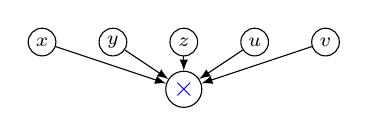
\begin{tikzpicture}[>=latex]
    \def\vars{{"$x$","$y$","$z$","$u$","$v$","$w$"}}
    
    \node[vert] (a) at (0, 0) {\textcolor{blue}{$\times$}};

    \foreach \i in {0, 1, ..., 4}{ 
        \node[vert] (b) at ({0.9 * (\i - 2)}, 0.6)
            {\scriptsize \pgfmathparse{\vars[\i]}\pgfmathresult};
        \draw[->] (b) -- (a);
    }
\end{tikzpicture}